\documentclass[12pt, notitlepage, final]{article}

\newcommand{\name}{Vince Coghlan}

%\usepackage[dvips]{graphics,color}
\usepackage{amsfonts}
\usepackage{amssymb}
\usepackage{amsmath}
\usepackage{latexsym}
\usepackage{enumerate}
\usepackage{amsthm}
\usepackage{nccmath}
\usepackage{setspace}
\usepackage[pdftex]{graphicx}
\usepackage{epstopdf}
\usepackage[siunitx]{circuitikz}
\usepackage{tikz}
\usepackage{float}
\usepackage{cancel}
\usepackage{setspace}
\usepackage{overpic}
\usepackage{mathtools}
\usepackage{listings}
\usepackage{color}
\usepackage{qtree}
%\usepackage{gensymb}

\usetikzlibrary{calc}
\usetikzlibrary{matrix}
\usetikzlibrary{positioning}

%\numberwithin{equation}{section}
\newcommand{\dbr}[1]{d_{\mbox{#1BR}}}
\newtheorem{lemma}{Lemma}
\newtheorem*{corollary}{Corollary}
\newtheorem{theorem}{Theorem}
\newtheorem{proposition}{Proposition}
\theoremstyle{definition}
\newtheorem{define}{Definition}

\newdimen\digitwidth{}
\settowidth\digitwidth{0}
\def~{\hspace{\digitwidth}}

\setlength{\parskip}{1pc}
\setlength{\parindent}{0pt}
\setlength{\topmargin}{-3pc}
\setlength{\textheight}{9.0in}
\setlength{\oddsidemargin}{0pc}
\setlength{\evensidemargin}{0pc}
\setlength{\textwidth}{6.5in}

\DeclareMathOperator*{\argmin}{arg\,min}

%absolute value code
\DeclarePairedDelimiter\abs{\lvert}{\rvert}%
\DeclarePairedDelimiter\norm{\lVert}{\rVert}
\makeatletter
\let\oldabs\abs{}
\def\abs{\@ifstar{\oldabs}{\oldabs*}}
%
\let\oldnorm\norm{}
\def\norm{\@ifstar{\oldnorm}{\oldnorm*}}
\makeatother

\def\dbar{{\mathchar'26\mkern-12mu d}}
%\def \P[x]{\Frac{\partial}{\partial x}}
%\def \D[x]{\Frac{d}{dx}}
\newcommand{\PD}[2]{\frac{\partial#1}{\partial#2}}
\newcommand{\PF}[1]{\frac{\partial}{\partial#1}}
\newcommand{\DD}[2]{\frac{d#1}{d#2}}
\newcommand{\DF}[1]{\frac{d}{d#1}}
\newcommand{\fix}[2]{\left(#1\right)_#2}
\newcommand{\ket}[1]{|#1\rangle}
\newcommand{\bra}[1]{\langle#1|}
\newcommand{\braket}[2]{\langle{} #1 | #2 \rangle}
\newcommand{\bopk}[3]{\langle{} #1 | #2 | #3 \rangle}
\newcommand{\Choose}[2]{\displaystyle{} {#1 \choose{} #2}}
\newcommand{\proj}[1]{\ket{#1}\bra{#1}}
\def\del{\vec{\nabla}}
\newcommand{\avg}[1]{\langle#1\rangle}
\newcommand{\piecewise}[4]{\left\{\beginProtected{array}{rl}#1&:#2\\#3&:#4\endProtected{array}\right.}
\newcommand{\systeme}[2]{\left\{\beginProtected{array}{rl}#1\\#2\endProtected{array}\right.}
\def\Godel{G$\ddot{\mbox{o}}$del}

\title{Log-Linear Learning Over Large Iterations in Sudoku Puzzles}
\date{\today}
\author{\name}

\begin{document}

\maketitle

Sudoku is a puzzle game played on a $9\times9$ board.  The goal is to have a unique occurence
of each didget in each row, column, and $3\times3$ square.  This can be modeled as a game with the
following parameters:
\begin{itemize}
  \item{Players $N=\{1,2,\ldots,n\}$ Where $n$ is the number of empty spaces}
  \item{Actions $a_i\in\mathcal{A}$ where an action is a number between 1 and 9 and the actions set $\mathcal{A}=a_1\times a_2\times\cdots\times a_n$}
  \item{Utility Functions $u_i:\mathcal{A}\rightarrow \mathbb{R}$ Where the utility will be the number of repetitions of a
    player's current action in a row, column, or square.}
    \begin{equation} \label{util}
      u_i(a)=u_\text{row$_i$}(a)+u_\text{column$_i$}(a)+u_\text{square$_i$}(a)
    \end{equation}
    where
    \[
      u_\text{row$_i$} = \sum_{j\in i_{row}}(a_j=a_i)
    \]
  \item{Welfare Function $W(a):\mathcal{A}\rightarrow\mathbb{R}$ where the global welfare of an action represents the global
    desireability of that action.  Let $a$ be the joint action $(a_i, a_{-i})$ where $a_{-i}=(a_1,\ldots,a_{i-1},a_{i+1},\ldots,a_n)$}
\end{itemize}
We are given the ability to design the welfare function however we would like.  Suppose that our objective is captured
by a function $\phi:\mathcal{A}\rightarrow\mathbb{R}$ where
\begin{equation} \label{potgame}
  u_i(a_i,a_{-i}) - u_i(a_i^*, a_{-i}) = \phi(a_i, a_{-i})-\phi(a_i^*, a_{-i})
\end{equation}
A $\phi$ satisfying~\eqref{potgame} will be known as a potential function~\cite{shapley94}.  It can be shown that the
game of Sudoku has a potential function when we define the utility as in~\eqref{util}.  We begin by assuming that the
potential function will take the form
\[
  \phi(a)=\phi_\text{row}(a)+\phi_\text{column}(a)+\phi_\text{square}(a)
\]
We can then show that
\[
  \phi_\text{row}(a) - \phi_\text{row}(a^*) = u_\text{row$_i$}(a) - u_\text{row$_i$}(a^*)
\]
And so on.  When a player changes his number, he increases the amount of repetitions of that number by $1$.  By doing this,
however, he has unintentionally increased the amount of repetitions of any other player preforming the same action, and
decreased the amount of repetitions of his old action.  One would expect that the potential function is the sum of utilities
of each player
\[
  \phi_{\text{row}}(a) = \sum_{i\in N}u_{\text{row$_i$}}(a)
\]
\[
  \phi_{\text{row}}(a) - \phi_{\text{row}}(a^*) = \sum_{i\in N}u_\text{row$_i$}(a) - \sum_{i\in N}u_\text{row$_i$}(a^*)
\]
\[
 = \sum_{i\in N}\sum_{j\in i_{row}}(a_j=a_i) - \sum_{i\in N}\sum_{j\in i_{row}}(a_j=a^*_i)
\]
\[
 = \sum_{j\in i_{row}}(a_j=a_i) - \sum_{j\in i_{row}}(a_j=a_i) + \sum_{i\in N\backslash  \{i\}}\sum_{j\in i_{row}}(a_j=a_i) - \sum_{i\in N\backslash \{i\}}\sum_{j\in i_{row}}(a_j=a^*_i)
\]
Now we will use the fact that an increase in $n$ in the repetitions of $a_i$ corresponds to an increase of 1 of $n$
other players playing $a_i$.  This means that:
\[
 = \sum_{j\in i_{row}}(a_j=a_i) - \sum_{j\in i_{row}}(a_j=a_i) + \sum_{j\in i_{row}}(a_j=a_i) - \sum_{j\in i_{row}}(a_j=a_i)
\]
\[
 = 2(\sum_{j\in i_{row}}(a_j=a_i) - \sum_{j\in i_{row}}(a_j=a_i))
\]
This tells us that we have twice the potential function, meaning our potential function for the row is
\[
  \phi_{\text{row}}(a) = \frac{1}{2}\sum_{i\in N}u_{\text{row$_i$}}(a)
\]
This can be easily extended to rows and columns to find:
\begin{equation} \label{potfun}
  \phi(a) = \frac{1}{2}\sum_{i\in N}u_i(a)
\end{equation}

Since sudoku has a potential function, the minimization of the potential is a pure equilibrium~\cite{neyman97}.
Since we cannot have a negative potential by our definition of the utility, and a potential of 0 means that
there are no repetitions in any row, column, or square, a pure Nash Equilibrium exists, and must be the solution
of the puzzle.

We have half of our problem laid out, the next part is to define a learning algorithm that will converge to this
equilibrium.  Current strategies being studied currently include fictitious play~\cite{shapley96}, log-linear
learning~\cite{blume93}, and the cournot best reply process~\cite{cournot38} among others.  Many of these
learning algorithms converge to a Nash equilibrium~\cite{marden12}.  It has been shown~\cite{young93} that Log-linear
learning provides us the fact that, in any exact potential game, log-linear learning will induce a Markov chain with
a unique stationary distrobution $\pi \in \Delta(\mathcal{A})$ of the form
\begin{equation} \label{usd}
  \pi_a=\frac{e^{\frac{1}{T} \phi(a)}}{\sum_{\tilde{a}\in\mathcal{A}}e^{\frac{1}{T}\phi(\tilde{a})}}
\end{equation}
Since $\phi$ is zero at the solutions, we know that the distrobutions of the system as $T\rightarrow 0$ will be
distributed on solutions to the sudoku puzzle.  We can see this behavior for some simple sudoku puzzles, for example,
this puzzle was solved in 28836 iterations, with a temperature of $T=0.5$.

\begin{figure}[H]
\begin{center}
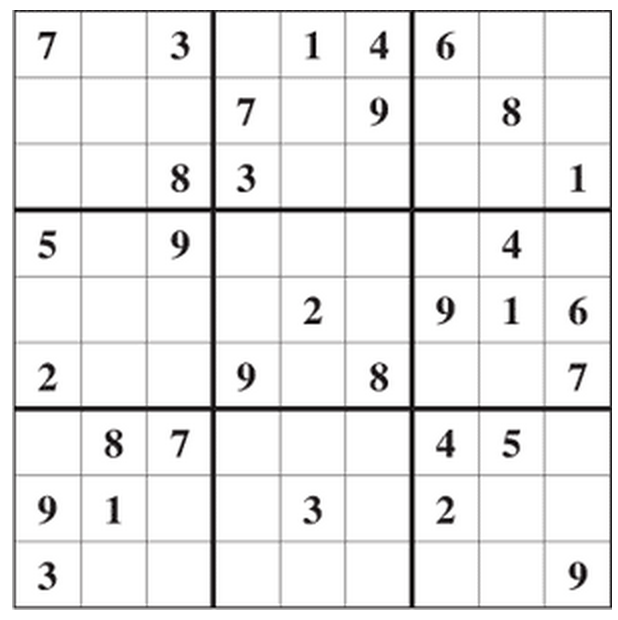
\includegraphics[width=5cm]{f1}
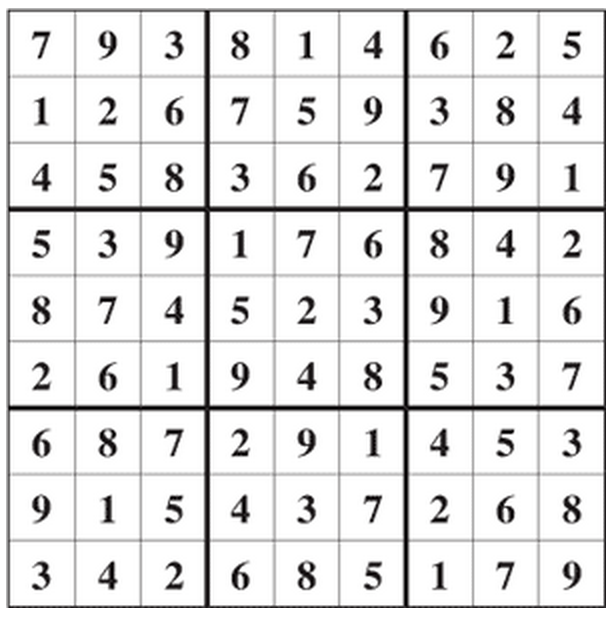
\includegraphics[width=5cm]{f2}
\end{center}
\end{figure}

The potential can be seen

\begin{figure}[H]
\begin{center}
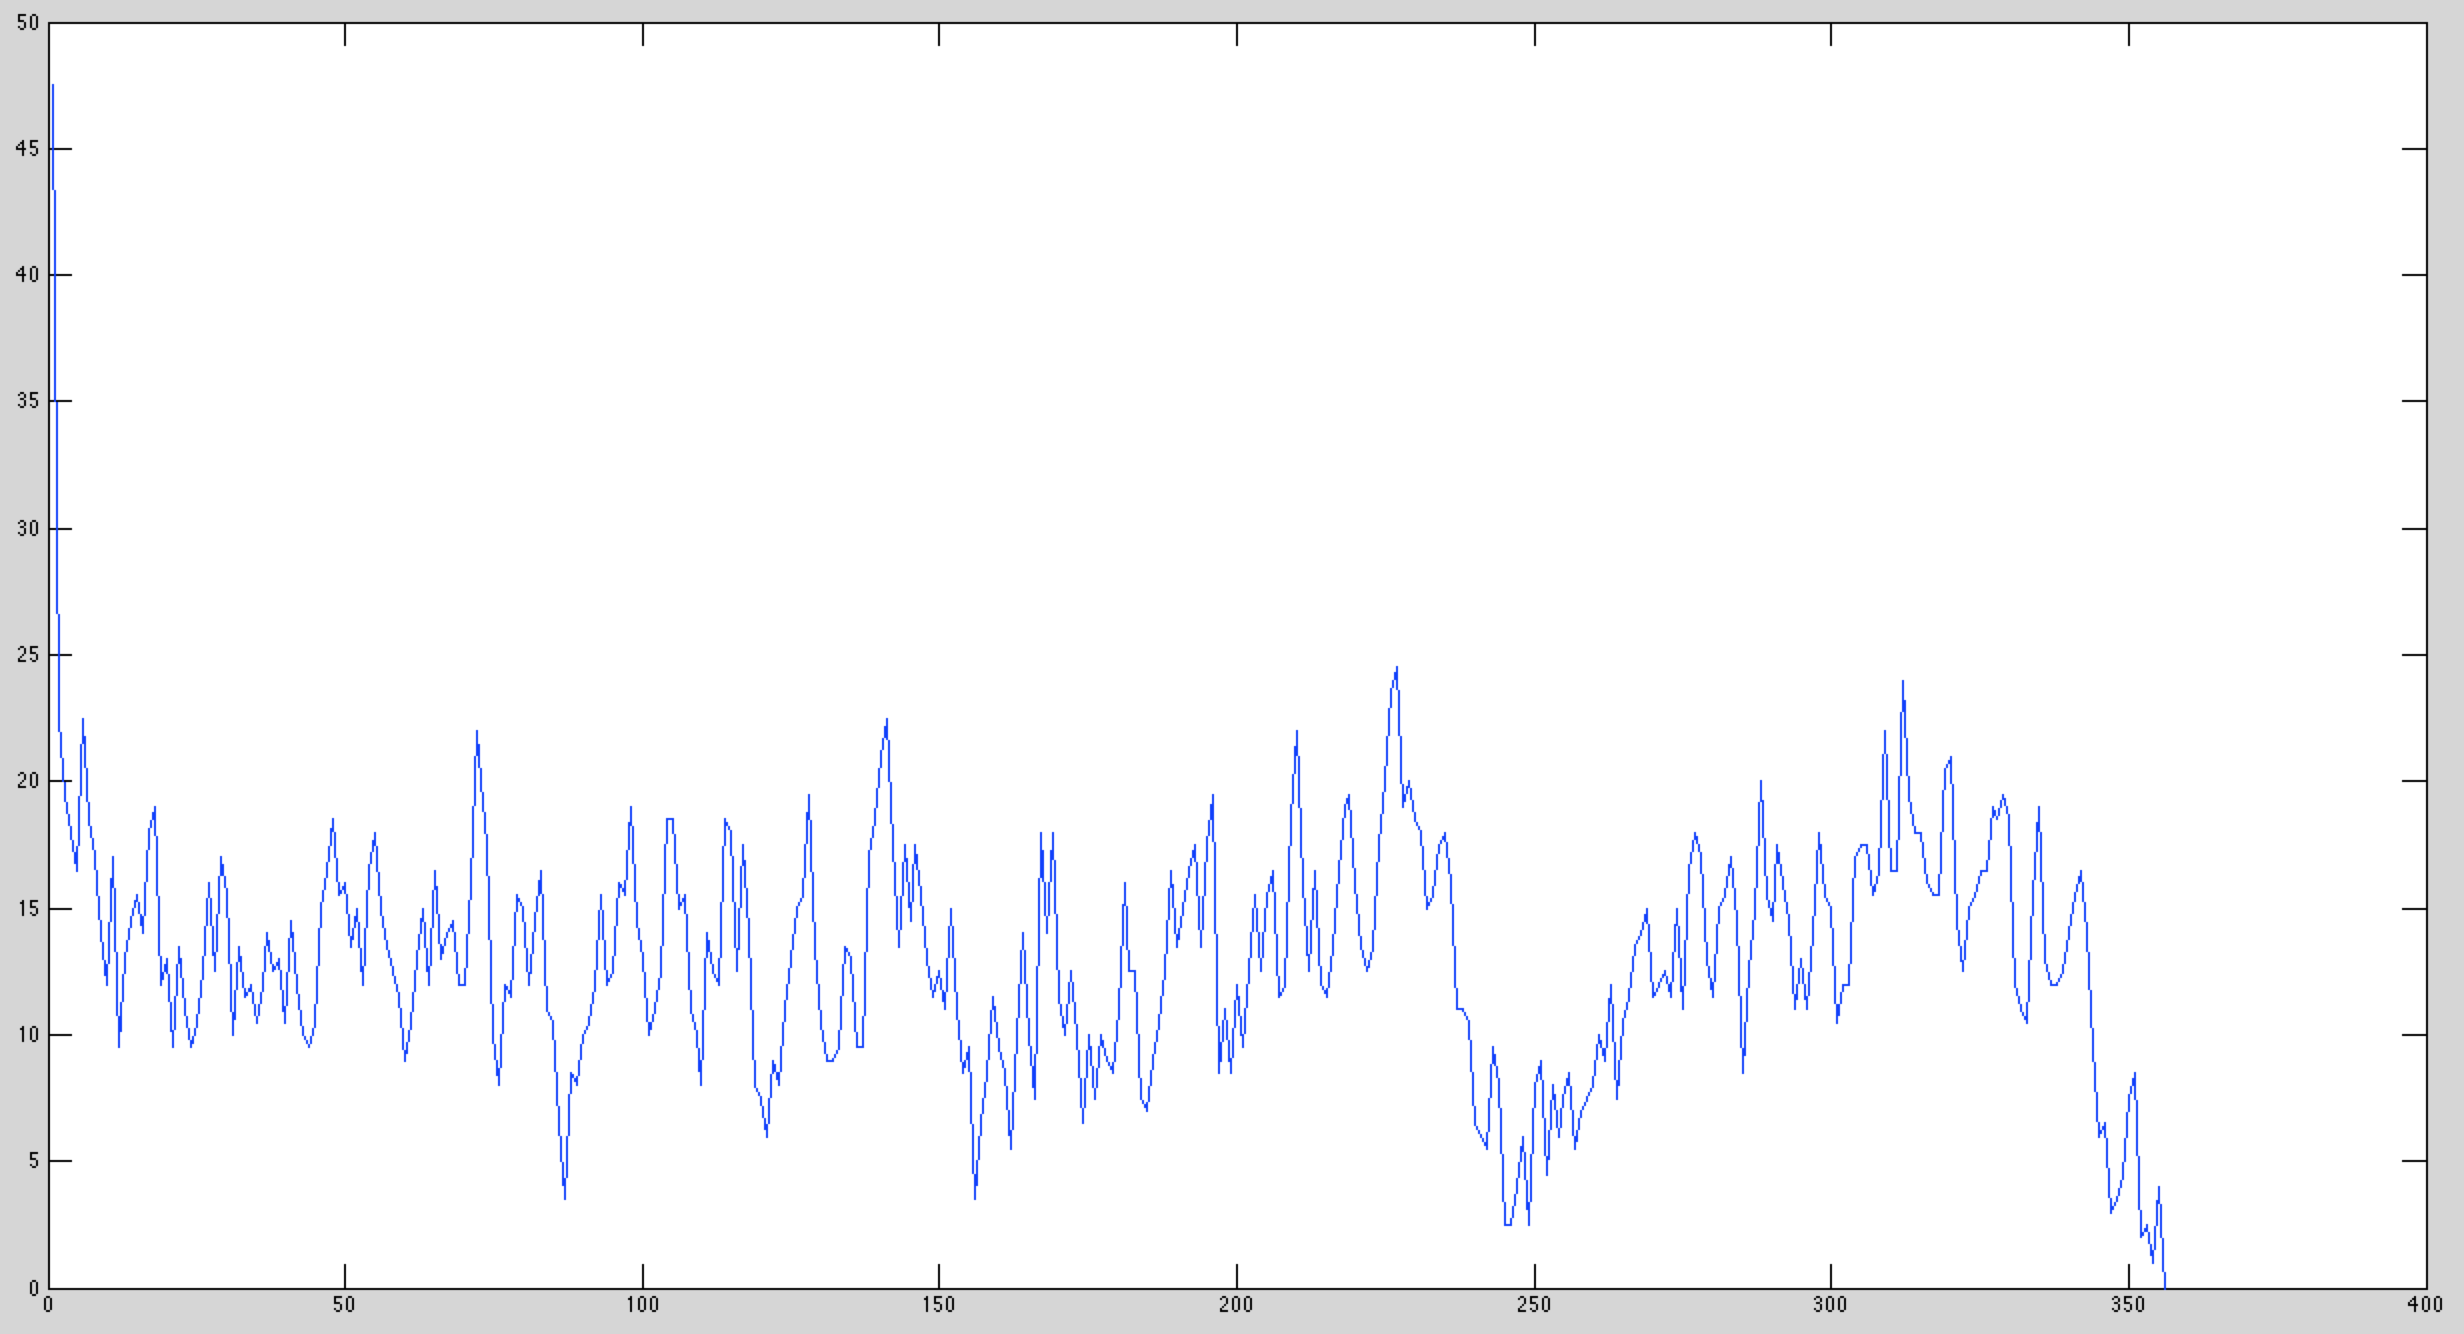
\includegraphics[width=12cm]{f3}
\end{center}
\end{figure}

You can see that once the potential is 0, we are done, and the puzzle is solved.  We can see a different story for a
different puzzle.

\newpage
\begin{thebibliography}{9}

  \bibitem{blume93}
  L. Blume,
  The statistical mechanics of strategic interaction.
  \emph{Games and Economic Behavior},
  pp. 387--424,
  1993.

  \bibitem{cournot38}
  A. Cournot,
  \emph{Recherches sur les principes math\'{e}matiques de la th\'{e}orie des richesses},
  Hachette,
  1838.

  \bibitem{neyman97}
  A. Neyman,
  Correlated Equilibrium and Potential Games.
  \emph{International Journal of Game Theory},
  pp. 223--227,
  1997.

  \bibitem{marden12}
  J. Marden and J. Shamma,
  Revisiting Log-Linear Learning: Asynchrony, Completeness and Payoff-Based Implementation
  \emph{Games and Economic Behavior},
  Volume 75, Issue 4, pp. 788--808,
  2012.

  \bibitem{shapley96}
  D. Monderer and L. Shapley,
  Fictitious Play Property for Games with Identical Interests.
  \emph{Journal of Economic Theory},
  Volume 68, pp. 258--265,
  1996

  \bibitem{shapley94}
  D. Monderer and L. Shapley,
  Potential Games.
  \emph{Games and Economic Behavior},
  Article No. 0044 pp. 124--143,
  1994.

\bibitem{young93}
  H.P. Young.
  The Evolution of Conventions.
  \emph{Econometrica},
  pp. 57--84,
  1993.


\end{thebibliography}

\end{document}
